\باب{برقرار حالت بدلتی رو}

\حصہ{سائن نما تفاعل}
سائن نما تفاعل سے مراد سائن تفاعل \عددی{\sin \theta} اور کو سائن تفاعل \عددی{\cos \theta} ہیں۔شکل \حوالہ{شکل_بدلتی_رو_سائن_تفاعل}-الف میں رداس \عددی{A_0} کے گول دائرے پر ایک نقطہ یکساں رفتار کے ساتھ، گھڑی کی گردش کی الٹ سمت میں، حرکت کر رہا ہے۔یہ دائرہ \اصطلاح{کارتیسی محدد}\فرہنگ{کارتیسی محدد}\حاشیہب{Cartesian coordinates}\فرہنگ{Cartesian coordinates} کے مرکز \عددی{(0,0)} پر پایا جاتا ہے۔لمحہ \عددی{t} پر زاویہ \عددی{\phase{aox}} کی قیمت \عددی{\theta} کے برابر ہے۔نقطے سے \عددی{x} محدد پر عمودی لکیر محدد کو  \عددی{x(t)}  پر ٹکراتی ہے جبکہ \عددی{y} محدد پر عمودی لکیر \عددی{y(t)} پر ٹکراتی ہے۔شکل کو دیکھتے ہوئے درج ذیل لکھا جا سکتا ہے جہاں \عددی{A_0} تفاعل کی چوٹی ہے جسے تفاعل کا \اصطلاح{حیطہ}\فرہنگ{حیطہ}\حاشیہب{amplitude}\فرہنگ{amplitude} کہتے ہیں۔
\begin{align}\label{مساوات_بدلتا_سائن_نما_تفاعل_الف}
y(t)&=A_0 \sin \theta
\end{align}
 گردش کرتا نقطہ ایک چکر میں \عددی{360^{\circ}} درجے کا زاویہ یعنی \عددی{2\pi} ریڈیئن طے کرتا ہے۔ایک چکر کاٹنے کے لئے درکار دورانیے کو \اصطلاح{دوری عرصہ}\فرہنگ{دوری عرصہ}\حاشیہب{time period}\فرہنگ{time period} کہتے ہیں جسے \عددی{T} سے ظاہر کیا جاتا ہے۔
%=========================
\ابتدا{مشق}
شکل \حوالہ{شکل_بدلتی_رو_سائن_تفاعل}-الف میں نقطہ ایک چکر \عددی{\SI{20}{\milli\second}} میں پورا کرتا ہے۔یہ نقطہ ایک سیکنڈ میں کتنے چکر پورا کرے گا۔یہ نقطہ ایک سیکنڈ میں کتنے ریڈیئن کا زاویہ طے کرتا ہے۔

جوابات:\عددی{50} چکر، \عددی{100\pi \, \si{\radian}}
\انتہا{مشق}
%========================

اگر ایک چکر کاٹنے کے لئے \عددی{T} سیکنڈ کا وقت درکار ہو تب ایک سیکنڈ میں چکروں کی تعداد  \عددی{\tfrac{1}{T}} ہو گی جسے \اصطلاح{تعدد}\فرہنگ{تعدد}\حاشیہب{frequency}\فرہنگ{frequency} کہتے اور \عددی{f} سے ظاہر کرتے ہیں۔
\begin{align}
f=\frac{1}{T}
\end{align}
تعدد کی اکائی \اصطلاح{ہرٹز}\فرہنگ{ہرٹز}\حاشیہب{Hertz}\فرہنگ{Hertz} ہے جسے \عددی{\si{\hertz}} سے ظاہر کیا جاتا ہے۔

ایک چکر \عددی{2\pi} ریڈیئن کو کہتے ہیں لہٰذا \عددی{f} چکر سے مراد \عددی{2\pi f} ریڈیئن کا زاویہ ہے۔یوں \عددی{f} تعدد پر گردش کرتا نقطہ ایک سیکنڈ میں \عددی{2\pi f} ریڈیئن کا زاویہ طے کرے گا یعنی اس کی \اصطلاح{زاویائی رفتار}\فرہنگ{زاویائی رفتار}\حاشیہب{angular speed}\فرہنگ{angular speed} کی قیمت \عددی{2\pi f} ہو گی۔زاویائی رفتار کو \عددی{\omega} سے ظاہر کیا جاتا ہے جبکہ اس کی اکائی ریڈیئن فی سیکنڈ \عددی{\si{\radian\per\second}} ہے۔
\begin{align}
\omega=2\pi f
\end{align}
زاویائی رفتار \عددی{\omega} سے گردش کرتا ہوا نقطہ \عددی{t} سیکنڈ میں \عددی{2\pi f t} ریڈیئن کا زاویہ طے کرے گا۔یوں اگر \عددی{t=0} پر نقطہ عین \عددی{x} محدد کے مثبت حصے پر ہو تب لمحہ \عددی{t} پر
\begin{align}
\theta=\omega t=2\pi f t
\end{align}
لکھا جائے گا۔یوں مساوات  \حوالہ{مساوات_بدلتا_سائن_نما_تفاعل_الف} کو
\begin{gather}
\begin{aligned}\label{مساوات_بدلتا_سائن_نما_تفاعل_ب}
y(t)&=A_0 \sin 2\pi f t\\
&=A_0\sin \frac{2\pi}{T}t\\
&=A_0 \sin \omega t
\end{aligned}
\end{gather}
لکھا جا سکتا ہے۔

برقی میدان میں \عددی{y(t)} وقت کے ساتھ بدلتے دباو یا وقت کے ساتھ بدلتی رو کو ظاہر کر سکتی ہے۔مساوات \حوالہ{مساوات_بدلتا_سائن_نما_تفاعل_ب} میں دیے تفاعل، جسے شکل \حوالہ{شکل_بدلتی_رو_سائن_تفاعل}-ب میں دکھایا گیا ہے،  کا آزاد متغیرہ وقت \عددی{t} ہے۔آپ دیکھ سکتے ہیں کہ یہ تفاعل ہر \عددی{T} سیکنڈ کے بعد اپنے آپ کو دہراتا ہے۔ اس حقیقت کو ریاضی میں درج ذیل لکھا جاتا ہے۔
\begin{align}
y(t+T)=y( t)
\end{align}
جس سے مراد یہ ہے کہ تفاعل کی قیمت لمحہ \عددی{t} اور لمحہ \عددی{t+T} پر برابر ہیں۔

\begin{figure}
\centering
\begin{subfigure}{0.5\textwidth}
\centering
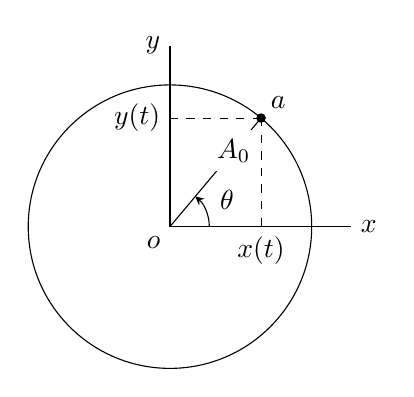
\begin{tikzpicture}
\pgfmathsetmacro{\ang}{50}
\pgfmathsetmacro{\rad}{1.8}
\pgfmathsetmacro{\xp}{\rad*cos(\ang)}
\pgfmathsetmacro{\yp}{\rad*sin(\ang)}
\draw[](0,0)--++(\rad+0.5,0)node[right]{$x$};
\draw[](0,0)--++(0,\rad+0.5)node[left]{$y$};
\draw[](0,0) circle (\rad);
\draw[fill](\ang:\rad) circle (1.5pt);
\draw(0,0)node[below left]{$o$}--++(\ang:\rad)node[pos=0.7,fill=white]{$A_0$}node[above right]{$a$};
\draw[-stealth] ([shift={(0:0.5)}]0,0) arc (0:\ang:0.5);
\draw(\ang/2:0.8)node{$\theta$};
\draw[dashed](\xp,\yp)--(\xp,0)node[below]{$x(t)$};
\draw[dashed](\xp,\yp)--(0,\yp)node[left]{$y(t)$};
\end{tikzpicture}
\caption*{الف}
\end{subfigure}
\begin{subfigure}{0.5\textwidth}
\centering
\begin{tikzpicture}
\begin{axis}[kStyleCircuitsA,small, xlabel=$t$, ylabel=$y(t)$, xtick={90,180,270,360},xticklabels={$\dfrac{T}{4}$,$\dfrac{T}{2}$,$\dfrac{3T}{2}$,$T$},ytick={-1,1},yticklabels={$-A_0$,$A_0$},
]
\addplot[domain=0:400,samples=100]{sin(x)};
\draw[gray,dashed](axis cs:0,1)--(axis cs:90,1);
\draw[gray,dashed](axis cs:0,-1)--(axis cs:270,-1);
\end{axis}%
\end{tikzpicture}%
\caption*{(ب)}
\end{subfigure}%
\begin{subfigure}{0.5\textwidth}
\centering
\begin{tikzpicture}
\begin{axis}[kStyleCircuitsA,small, xlabel=$\omega t$, ylabel=$y(\omega t)$, xtick={90,180,270,360},xticklabels={$\dfrac{\pi}{2}$,$\pi$,$\dfrac{3\pi}{2}$,$2\pi$},ytick={-1,1},yticklabels={$-A_0$,$A_0$},
]
\addplot[domain=0:400,samples=100]{sin(x)};
\draw[gray,dashed](axis cs:0,1)--(axis cs:90,1);
\draw[gray,dashed](axis cs:0,-1)--(axis cs:270,-1);
\end{axis}%
\end{tikzpicture}%
\caption*{(پ)}
\end{subfigure}%
\caption{سائن تفاعل۔}
\label{شکل_بدلتی_رو_سائن_تفاعل}
\end{figure}%

مساوات \حوالہ{مساوات_بدلتا_سائن_نما_تفاعل_ب} کے خط کو \عددی{\omega t} کے ساتھ بھی کھینچا جا سکتا ہے۔ایسا ہی شکل \حوالہ{شکل_بدلتی_رو_سائن_تفاعل}-پ میں دکھایا گیا ہے جہاں سے واضح ہے کہ یہ تفاعل ہر \عددی{2\pi} ریڈیئن کے بعد اپنے آپ کو دہراتا ہے۔
%====================
\ابتدا{مشق}
شکل \حوالہ{شکل_بدلتی_رو_سائن_تفاعل}-الف میں گردش کرتا نقطہ \عددی{\SI{0.2}{\second}} میں \عددی{40^{\circ}} کا زاویہ طے کرتا ہے۔زاویائی رفتار، تعدد اور دوری عرصہ دریافت کریں۔

جوابات:\عددی{\omega=\tfrac{10\pi}{9}\,\si{\radian\per\second}}، \عددی{f=\SI{1.8}{\hertz}}، \عددی{T=\frac{5}{9} \, \si{\second}}
\انتہا{مشق}
%=================

شکل \حوالہ{شکل_بدلتا_لمحہ_صفر_پر_مقام_الفا_ہے} میں عمومی صورت حال دکھائی گئی ہے جہاں \عددی{\omega} زاویائی رفتار سے گردش کرتا نقطہ، لمحہ \عددی{t=0} پر  زاویہ \عددی{\alpha} پر پایا جاتا ہے۔یہ نقطہ وقت \عددی{t} کے دوران \عددی{\omega t} زاویہ طے کرتے ہوئے \عددی{\theta=\omega t+\alpha} پہنچ جائے گا لہٰذا اس کے لئے
\begin{align}\label{مساوات_بدلتا_سائن_نما_تفاعل_پ}
y(t)=A_0 \sin(\omega t +\alpha)
\end{align}
لکھا جا سکتا ہے جہاں \عددی{\alpha} کو \اصطلاح{زاویائی ہٹاو}\فرہنگ{زاویائی ہٹاو}\حاشیہب{phase angle}\فرہنگ{phase angle} کہتے ہیں۔شکل \حوالہ{شکل_بدلتا_لمحہ_صفر_پر_مقام_الفا_ہے}-ب میں مساوات \حوالہ{مساوات_بدلتا_سائن_نما_تفاعل_ب} اور مساوات \حوالہ{مساوات_بدلتا_سائن_نما_تفاعل_پ} کو دکھایا گیا ہے۔آپ دیکھ سکتے ہیں کہ مساوات \حوالہ{مساوات_بدلتا_سائن_نما_تفاعل_ب} سے  مساوات \حوالہ{مساوات_بدلتا_سائن_نما_تفاعل_پ} \عددی{\alpha} ریڈیئن \اصطلاح{آگے}\فرہنگ{آگے}\حاشیہب{lead}\فرہنگ{lead} ہے۔ یہ بھی کہا جا سکتا ہے کہ مساوات \حوالہ{مساوات_بدلتا_سائن_نما_تفاعل_پ} سے مساوات \حوالہ{مساوات_بدلتا_سائن_نما_تفاعل_پ} \عددی{\alpha} ریڈیئن \اصطلاح{پیچھے}\فرہنگ{پیچھے}\حاشیہب{lag}\فرہنگ{lag} ہے۔

\begin{figure}
\centering
\begin{subfigure}{0.5\textwidth}
\centering
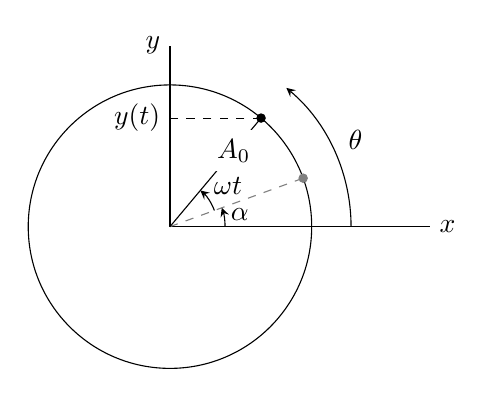
\begin{tikzpicture}
\pgfmathsetmacro{\angA}{20}
\pgfmathsetmacro{\angB}{50}
\pgfmathsetmacro{\rad}{1.8}
\pgfmathsetmacro{\xp}{\rad*cos(\angB)}
\pgfmathsetmacro{\yp}{\rad*sin(\angB)}
\draw[](0,0)--++(\rad+1.5,0)node[right]{$x$};
\draw[](0,0)--++(0,\rad+0.5)node[left]{$y$};
\draw[](0,0) circle (\rad);
\draw[gray,fill](\angA:\rad) circle (1.5pt);
\draw[fill](\angB:\rad) circle (1.5pt);
\draw[dashed,gray](0,0)--++(\angA:\rad);
\draw(0,0)--++(\angB:\rad)node[pos=0.7,fill=white]{$A_0$};
\draw[dashed](\xp,\yp)--(0,\yp)node[left]{$y(t)$};
%angles
\draw[-stealth] ([shift={(0:0.7)}]0,0) arc (0:\angA:0.7);
\draw(\angA/2:0.9)node{$\alpha$};
\draw[-stealth] ([shift={(\angA:0.6)}]0,0) arc (\angA:\angB:0.6);
\draw(\angA/2+\angB/2:0.9)node{$\omega t$};
\draw[-stealth] ([shift={(0:\rad+0.5)}]0,0) arc (0:\angB:\rad+0.5);
\draw(\angB/2:\rad+0.8)node{$\theta$};
\end{tikzpicture}
\caption*{(الف)}
\end{subfigure}%
\begin{subfigure}{0.5\textwidth}
\centering
\begin{tikzpicture}
\begin{axis}[kStyleCircuitsA,small,xlabel=$t$, ylabel=$y(t)$,ytick={1},yticklabels={$A_0$},xtick={180,360},xticklabels={$\pi$,$2\pi$},]
\addplot[domain=0:370,samples=100,dashed]{sin(x)}node[pos=0.42,pin={[font=\small]10:${A_0\sin \omega t}$},inner sep=0pt]{};
\addplot[domain=-60:320,samples=100]{sin(x+60)}node[pos=0.35,pin={[pin distance=0.75cm,font=\small]10:${A_0\sin (\omega t+\alpha)}$},inner sep=0pt]{};
\draw(axis cs:-60,-0.1)--(axis cs:-60,-0.3);
\draw[stealth-](axis cs:0,-0.2)--(axis cs:30,-0.2);
\draw[stealth-](axis cs:-60,-0.2)--(axis cs:-80,-0.2)--(axis cs:-100,-0.4)node[below]{$\alpha$};
\end{axis}
\end{tikzpicture}
\caption*{(ب) زاویائی ہٹاو۔}
\end{subfigure}%
\caption{لمحہ \عددی{t=0} پر زاویہ \عددی{\alpha} ہے۔}
\label{شکل_بدلتا_لمحہ_صفر_پر_مقام_الفا_ہے}
\end{figure}

